
%%%%%%%%%%%%%%%%%%%%%%%%%%%%%%%%%%%%%%%%%
% Short Sectioned Assignment LaTeX Template Version 1.0 (5/5/12)
% This template has been downloaded from: http://www.LaTeXTemplates.com
% Original author:  Frits Wenneker (http://www.howtotex.com)
% License: CC BY-NC-SA 3.0 (http://creativecommons.org/licenses/by-nc-sa/3.0/)
%%%%%%%%%%%%%%%%%%%%%%%%%%%%%%%%%%%%%%%%%

%----------------------------------------------------------------------------------------
%	PACKAGES AND OTHER DOCUMENT CONFIGURATIONS
%----------------------------------------------------------------------------------------

\documentclass[paper=a4, fontsize=11pt]{scrartcl} % A4 paper and 11pt font size

% ---- Entrada y salida de texto -----

\usepackage[T1]{fontenc} % Use 8-bit encoding that has 256 glyphs
\usepackage[utf8]{inputenc}
%\usepackage{fourier} % Use the Adobe Utopia font for the document - comment this line to return to the LaTeX default

% ---- Idioma --------

\usepackage[spanish, es-tabla]{babel} % Selecciona el español para palabras introducidas automáticamente, p.ej. "septiembre" en la fecha y especifica que se use la palabra Tabla en vez de Cuadro

% ---- Otros paquetes ----

\usepackage{url} % ,href} %para incluir URLs e hipervínculos dentro del texto (aunque hay que instalar href)
\usepackage{amsmath,amsfonts,amsthm} % Math packages
%\usepackage{graphics,graphicx, floatrow} %para incluir imágenes y notas en las imágenes
\usepackage{graphics,graphicx, float} %para incluir imágenes y colocarlas
\usepackage{movie15}

% Para hacer tablas comlejas
%\usepackage{multirow}
%\usepackage{threeparttable}

%\usepackage{sectsty} % Allows customizing section commands
%\allsectionsfont{\centering \normalfont\scshape} % Make all sections centered, the default font and small caps

\usepackage{fancyhdr} % Custom headers and footers

\pagestyle{fancyplain} % Makes all pages in the document conform to the custom headers and footers
\fancyhead{} % No page header - if you want one, create it in the same way as the footers below
\fancyfoot[L]{} % Empty left footer
\fancyfoot[C]{} % Empty center footer
\fancyfoot[R]{\thepage} % Page numbering for right footer
\renewcommand{\headrulewidth}{0pt} % Remove header underlines
\renewcommand{\footrulewidth}{0pt} % Remove footer underlines
\setlength{\headheight}{13.6pt} % Customize the height of the header

\numberwithin{equation}{section} % Number equations within sections (i.e. 1.1, 1.2, 2.1, 2.2 instead of 1, 2, 3, 4)
\numberwithin{figure}{section} % Number figures within sections (i.e. 1.1, 1.2, 2.1, 2.2 instead of 1, 2, 3, 4)
\numberwithin{table}{section} % Number tables within sections (i.e. 1.1, 1.2, 2.1, 2.2 instead of 1, 2, 3, 4)

\setlength\parindent{0pt} % Removes all indentation from paragraphs - comment this line for an assignment with lots of text

\newcommand{\horrule}[1]{\rule{\linewidth}{#1}} % Create horizontal rule command with 1 argument of height
\usepackage[breaklinks=true]{hyperref}
\usepackage{bookmark}
\usepackage{wasysym}
\usepackage{subcaption}
\usepackage[dvipsnames]{xcolor}
\usepackage{amssymb}
\usepackage{color}
\usepackage{listings}
\usepackage{upgreek} % para poner letras griegas sin cursiva
\usepackage{cancel} % para tachar
\usepackage{mathdots} % para el comando \iddots
\usepackage{mathrsfs} % para formato de letra
\usepackage{stackrel} % para el comando \stackbin
\lstdefinestyle{cmas}
{ %
	language=C++,                % elegir el lenguaje del código
	stringstyle=\color{blue}\ttfamily,,
	basicstyle=\normalsize\ttfamily,       % el tamaño del font a usar para el código
	numbers=left,                   % dónde poner los números de línea 
	numberstyle=\footnotesize,      % tamaño de font usados para los números de línea 
	stepnumber=1,                   % el paso de numeración
	numbersep=8pt,                  % distancia del numero de línea y la línea
	backgroundcolor=\color{white},  % color de fondo, para usarlo hay que agregar  \usepackage{color}
	showspaces=false,               % mostrar espacios en blanco ?
	showstringspaces=false,         % subrayar espacios con cadenas?   
	 showtabs=false,                 % mostrar taba usando cadenas? 
	frame=single,           			% enmarcar el código?  
	tabsize=2,          				% sets default tabsize to 2 spaces?
	keywordstyle=\color{MidnightBlue}\ttfamily\bfseries,
	commentstyle=\color{OliveGreen}\ttfamily,
	morecomment=[l][\color{OliveGreen}]{\#},
	captionpos=b,           % sets the caption-position to bottom?
	breaklines=true,        % sets automatic line breaking?
	breakatwhitespace=false,    % sets if automatic breaks should only happen at whitespace ?
	title=\lstname,
	escapeinside={\%*}{*)}          % if you want to add a comment within your code
}

\lstdefinestyle{payt}
{ %
	language=Python,                % elegir el lenguaje del código
	stringstyle=\color{blue}\ttfamily,,
	basicstyle=\normalsize\ttfamily,       % el tamaño del font a usar para el código
	numbers=left,                   % dónde poner los números de línea 
	numberstyle=\footnotesize,      % tamaño de font usados para los números de línea 
	stepnumber=1,                   % el paso de numeración
	numbersep=8pt,                  % distancia del numero de línea y la línea
	backgroundcolor=\color{white},  % color de fondo, para usarlo hay que agregar  \usepackage{color}
	showspaces=false,               % mostrar espacios en blanco ?
	showstringspaces=false,         % subrayar espacios con cadenas?   
	showtabs=false,                 % mostrar taba usando cadenas? 
	frame=single,           			% enmarcar el código?  
	tabsize=2,          				% sets default tabsize to 2 spaces?
	keywordstyle=\color{MidnightBlue}\ttfamily\bfseries,
	commentstyle=\color{OliveGreen}\ttfamily,
	morecomment=[l][\color{OliveGreen}]{\#},
	captionpos=b,           % sets the caption-position to bottom?
	breaklines=true,        % sets automatic line breaking?
	breakatwhitespace=false,    % sets if automatic breaks should only happen at whitespace ?
	title=\lstname,
	escapeinside={\%*}{*)}          % if you want to add a comment within your code
}

\definecolor{light-gray}{gray}{0.85}

\lstdefinestyle{fich}
{ %
	language=Bash,                % elegir el lenguaje del código
	stringstyle=\color{black}\texttt,
	basicstyle=\normalsize\ttfamily,       % el tamaño del font a usar para el código	
	numbers=left,                   % dónde poner los números de línea 
	numberstyle=\footnotesize,      % tamaño de font usados para los números de línea 
	stepnumber=1,                   % el paso de numeración
	numbersep=8pt,                  % distancia del numero de línea y la línea
	backgroundcolor=\color{light-gray},  % color de fondo, para usarlo hay que agregar  \usepackage{color}
	showspaces=false,               % mostrar espacios en blanco ?
	showstringspaces=false,         % subrayar espacios con cadenas?   
	showtabs=false,                 % mostrar taba usando cadenas? 
%	frame=single,           			% enmarcar el código?  
	tabsize=2,          				% sets default tabsize to 2 spaces?
	captionpos=b,           % sets the caption-position to bottom?
	breaklines=true,        % sets automatic line breaking?
	breakatwhitespace=false,    % sets if automatic breaks should only happen at whitespace ?
	title=\lstname,
	escapeinside={\%*}{*)}          % if you want to add a comment within your code
}

\lstset{literate=
  {á}{{\'a}}1 {é}{{\'e}}1 {í}{{\'i}}1 {ó}{{\'o}}1 {ú}{{\'u}}1
  {Á}{{\'A}}1 {É}{{\'E}}1 {Í}{{\'I}}1 {Ó}{{\'O}}1 {Ú}{{\'U}}1
  {à}{{\`a}}1 {è}{{\`e}}1 {ì}{{\`i}}1 {ò}{{\`o}}1 {ù}{{\`u}}1
  {À}{{\`A}}1 {È}{{\'E}}1 {Ì}{{\`I}}1 {Ò}{{\`O}}1 {Ù}{{\`U}}1
  {ä}{{\"a}}1 {ë}{{\"e}}1 {ï}{{\"i}}1 {ö}{{\"o}}1 {ü}{{\"u}}1
  {Ä}{{\"A}}1 {Ë}{{\"E}}1 {Ï}{{\"I}}1 {Ö}{{\"O}}1 {Ü}{{\"U}}1
  {â}{{\^a}}1 {ê}{{\^e}}1 {î}{{\^i}}1 {ô}{{\^o}}1 {û}{{\^u}}1
  {Â}{{\^A}}1 {Ê}{{\^E}}1 {Î}{{\^I}}1 {Ô}{{\^O}}1 {Û}{{\^U}}1
  {œ}{{\oe}}1 {Œ}{{\OE}}1 {æ}{{\ae}}1 {Æ}{{\AE}}1 {ß}{{\ss}}1
  {ű}{{\H{u}}}1 {Ű}{{\H{U}}}1 {ő}{{\H{o}}}1 {Ő}{{\H{O}}}1
  {ç}{{\c c}}1 {Ç}{{\c C}}1 {ø}{{\o}}1 {å}{{\r a}}1 {Å}{{\r A}}1
  {€}{{\EUR}}1 {£}{{\pounds}}1
  {ñ}{{\~n}}1
}

\hypersetup{
    colorlinks=true,
    linkcolor=black,
    filecolor=magenta,      
    urlcolor=blue,
    pdftitle={ISE: Práctica 3 - Mario Rodríguez Ruiz},
    bookmarks=true,
    citecolor=blue,
}



%----------------------------------------------------------------------------------------
%	TÍTULO Y DATOS DEL ALUMNO
%----------------------------------------------------------------------------------------

\title{	
\normalfont \normalsize 
\textsc{\textbf{Ingeniería de Servidores (2016-2017)} \\ Subgrupo A1 \\ Grado en Ingeniería Informática\\ Universidad de Granada} \\ [25pt] % Your university, school and/or department name(s)
\horrule{0.5pt} \\[0.4cm] % Thin top horizontal rule
\huge Práctica 1: Instalación de Sistemas Operativos para servidores y
configuración de RAID1 \\ % The assignment title
\horrule{2pt} \\[0.5cm] % Thick bottom horizontal rule
}

\author{Mario Rodríguez Ruiz} % Nombre y apellidos

\date{\normalsize\today} % Incluye la fecha actual

%----------------------------------------------------------------------------------------
% DOCUMENTO
%----------------------------------------------------------------------------------------

\begin{document}

\maketitle % Muestra el Título

\newpage %inserta un salto de página

\tableofcontents % para generar el índice de contenidos

\listoffigures

\newpage

%----------------------------------------------------------------------------------------
%	Cuestión 1
%----------------------------------------------------------------------------------------

\section{Tipos de virtualización.}
\emph{\textbf{¿Qué modos y/o tipos de “virtualización” existen?}}

Existen dos tipos principales de virtualización:

\subsection{Virtualización de plataforma}
	
	Este tipo de virtualización crea una máquina virtual por medio de la utilización conjunta de software y hardware. Ésta se ejecuta a través de un software y en el que aparenta ser un entorno computacional.
	
	En este entorno se encuentran distintos tipos:
	\begin{itemize}
		\item \textbf{Virtualización nativa o completa}.
		
		Simula un hardware básico que permite su ejecución sobre el mismo CPU que el anfitrión a través de un sistema operativo invitado sin modificaciones. Ejemplo: Microsoft Virtual PC
		
		\item \textbf{Paravirtualización}.
		
		 Los SOs invitados se ejecutan sobre otro SO que actúa como hypervisor, éstos deben comunicarse con él para su correcta virtualización. Por lo que no tiene por qué simular el hardware.
		 Ejemplo: Xen en CPU estándar
		
		\item \textbf{Virtualización asistida por hardware.}
		
		Parte con la base de una virtualización completa con el añadido de que el procesador contribuye con la ejecución. Ejemplo: VirtualBox, VMware... etc
		
		\item \textbf{Virtualización a nivel de sistema operativo.}
		
		El hardware a nivel de SO es virtualizado por el SO anfitrión lo que permite que distintos SO virtuales se ejecuten de forma separada en un único medio físico.
		Ejemplo: Linux-VServer
		
		\item \textbf{Emulación.}
		
		Simula un hardware completo y permite ejecutar aplicaciones en una plataforma distinta para la que se creó. Ejemplo: PearPC (emulador PowerPC para x86).
		
	\end{itemize}
	
\subsection{Virtualización de recursos}
	
	Este tipo de virtualización es la que engloba volúmenes de almacenamiento, recursos de red y espacios de nombres para estacionarlos en una misma simulación de recursos.
	
	\begin{itemize}
		\item Redes Privadas Virtuales (VPN)
		\item Discos RAID y gestores de volúmenes (como Linux LVM).
		\item Sistemas multiprocesador y multinúcleo
	\end{itemize}

\subsection{Otros}
	\begin{itemize}
		\item \textbf{Virtualización de aplicaciones}
		
		Una aplicación es ejecutada en una máquina virtual dedicada a ello por medio de recursos locales que le proporcionan todos los componentes que necesita.
		Existe una capa entre el SO y la aplicación encargada de eliminar conflictos entre éstos.
		Ejemplo: Java Virtual Machine de Sun (JVM)
		
		\item \textbf{Virtualización de escritorio}
		
		Es la implementación de un escritorio como servicio, es decir, se aloja un SO de escritorio internamente en la máquina virtual.
		Ejemplos: VDI(Oracle, Red Hat)
		
	\end{itemize}

\cite{enlace3, enlace2, enlace1}
%----------------------------------------------------------------------------------------
%	Cuestión 2
%----------------------------------------------------------------------------------------

\section{Comparativa de proveedores VPS}
\emph{\textbf{Muestre los precios y características de varios proveedores de
		VPS (Virtual Private Server) y compare con el precio de servidores
		dedicados (administrados y no administrados). Comente diferencias.}}
	
	\subsection{Virtual Private Servers}
	\begin{figure}[H] %con el [H] le obligamos a situar aquí la figura
		\centering
		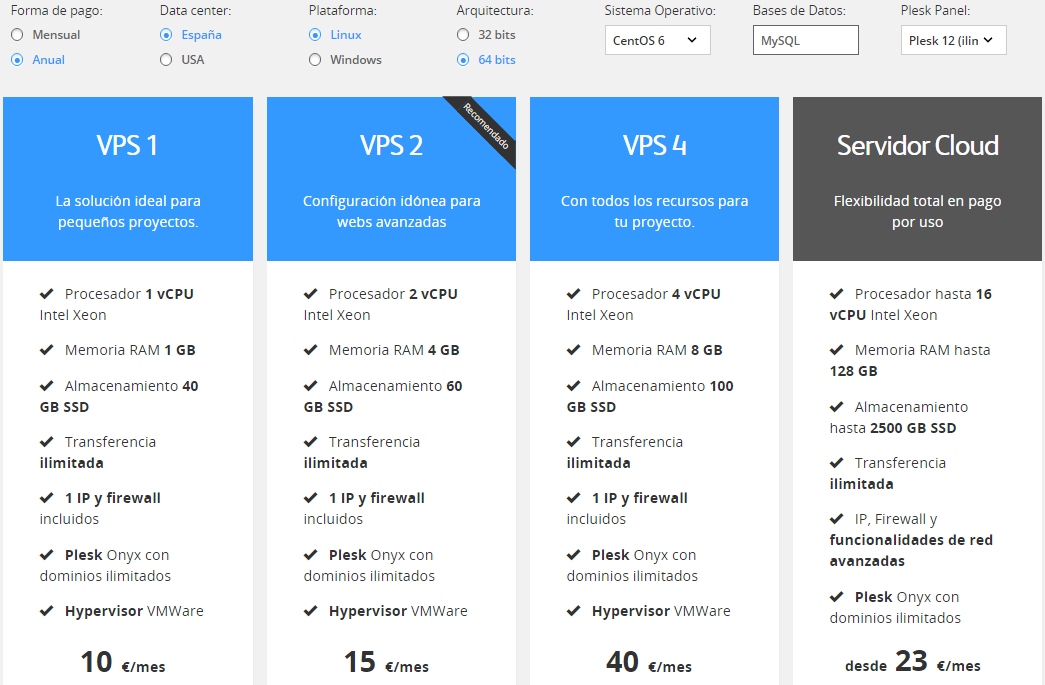
\includegraphics[scale=0.5]{figuras/foto1.png} 
		\caption{Diferentes configuraciones VPS Arsys \cite{figura1}} \label{fig:figura1}
	\end{figure}

	\begin{figure}[H] %con el [H] le obligamos a situar aquí la figura
		\centering
		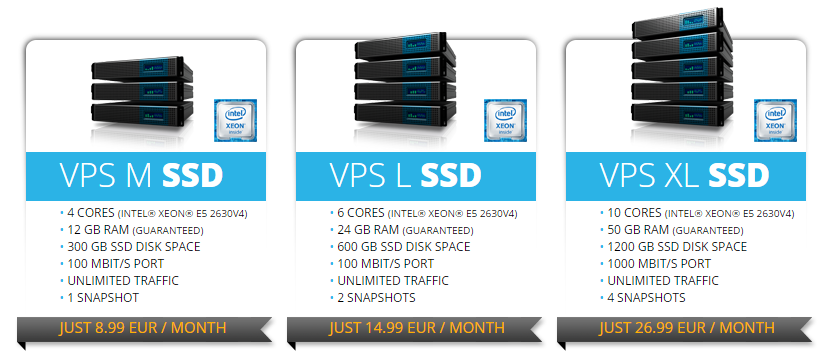
\includegraphics[scale=0.7]{figuras/contabo.png} 
		\caption{Diferentes configuraciones VPS Contabo \cite{figura2}} \label{fig:figura2}
	\end{figure}

	\begin{figure}[H] %con el [H] le obligamos a situar aquí la figura
		\centering
		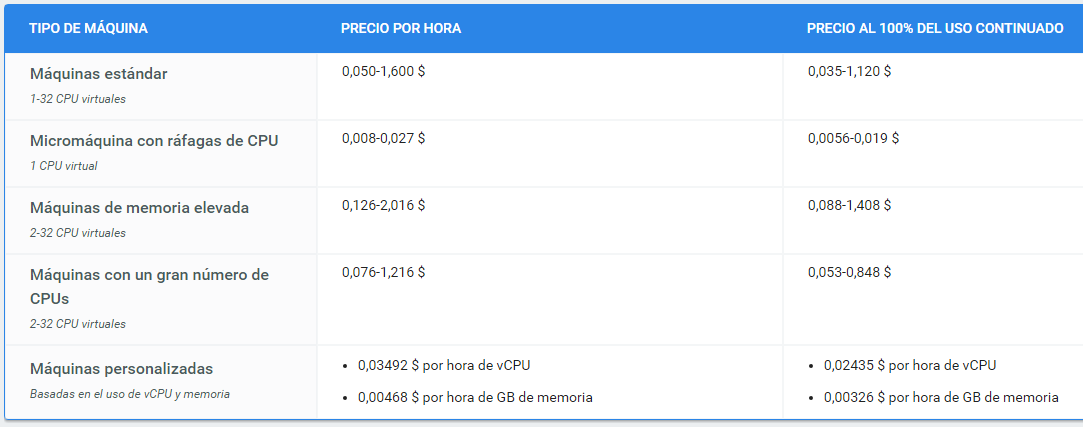
\includegraphics[scale=0.5]{figuras/google.png} 
		\caption{Diferentes configuraciones VPS Google \cite{figura3}} \label{fig:figura3}
	\end{figure}
	
	\subsection{Servidores dedicados administrados}
	\begin{figure}[H] %con el [H] le obligamos a situar aquí la figura
		\centering
		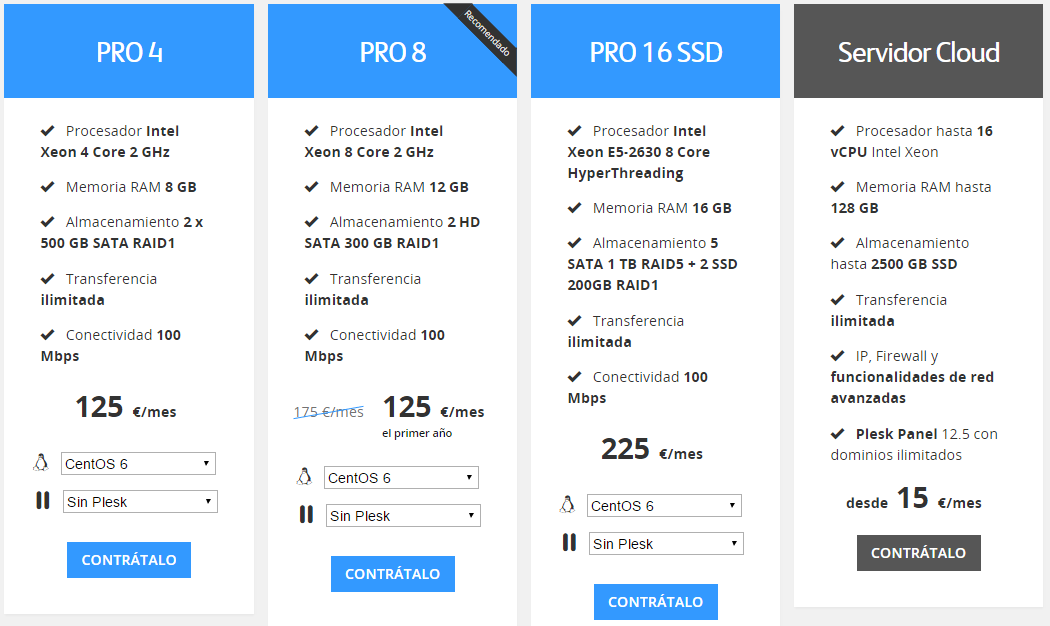
\includegraphics[scale=0.5]{figuras/arsysDed.png} 
		\caption{Servidores dedicados Arsys \cite{figura4}} \label{fig:figura4}
	\end{figure}
	\begin{figure}[H] %con el [H] le obligamos a situar aquí la figura
		\centering
		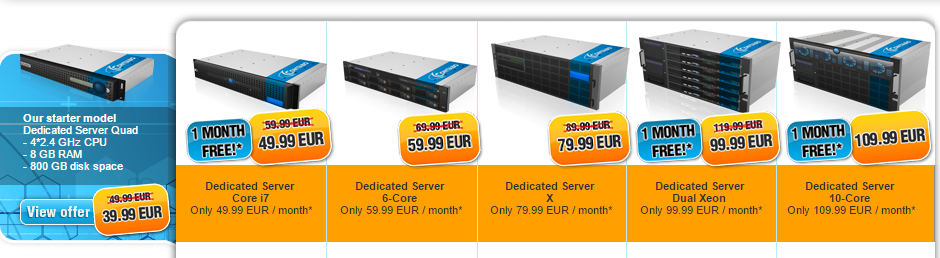
\includegraphics[scale=0.6]{figuras/contaboDed.png} 
		\caption{Servidores dedicados Contabo \cite{figura5}} \label{fig:figura5}
	\end{figure}
	
	\subsection{Servidores dedicados no administrados}
	\begin{figure}[H] %con el [H] le obligamos a situar aquí la figura
		\centering
		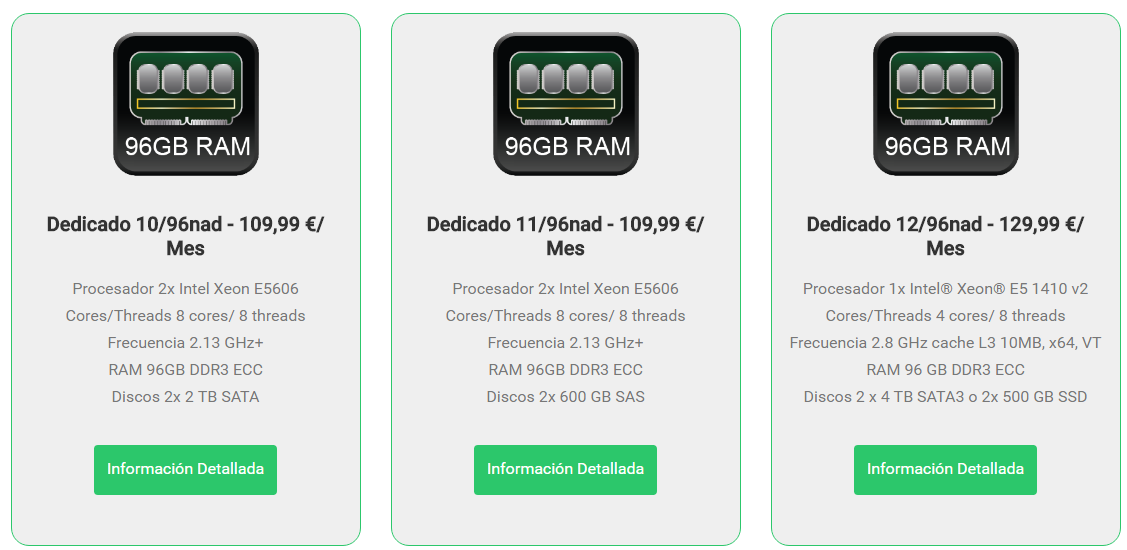
\includegraphics[scale=0.5]{figuras/noAdmin.png} 
		\caption{Servidores dedicados no administrados Rubinhost \cite{figura6}} \label{fig:figura6}
	\end{figure}
	\begin{figure}[H] %con el [H] le obligamos a situar aquí la figura
		\centering
		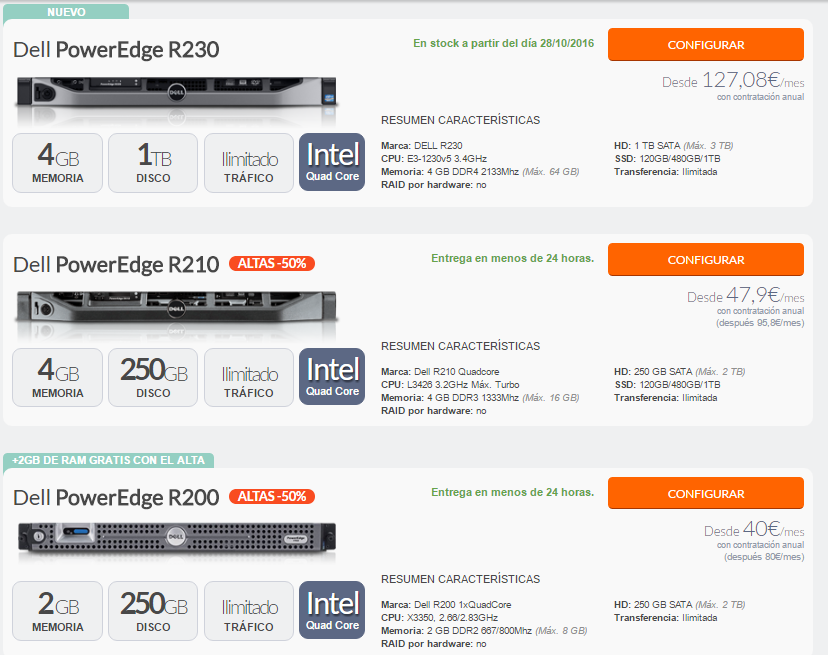
\includegraphics[scale=0.5]{figuras/noAd.png} 
		\caption{Servidores dedicados no administrados Dinahosting \cite{figura7}} \label{fig:figura7}
		\end{figure}
	
	\subsection{VPS vs Servidores dedicados}
	
	Antes de hacer la comparativa entre ambos hay que tener clara la diferencia entre
	los dedicados administrados y los dedicados NO administrados. Para ello se debe conocer que existen ventajas evidentes de un servidor NO administrado sobre un administrado. 
	
	Desde el punto de vista técnico el usuario tiene acceso al 100\% del servidor, de forma que se puede decidir la configuración y bajo unas condiciones, además, más económicas. Sin embargo, todo ello equivale a que el soporte no es tan amplio por lo que se requieren conocimientos avanzados de administración de servidores.\cite{enlace4}
	
	Desde el punto de vista económico también hay una diferencia clara. Como se puede asegurar observando las figuras \ref{fig:figura6} y \ref{fig:figura4}, los servicios no administrados ofrecen un precio muy por debajo del de los administrados. 
	Se puede ver en la Figura \ref{fig:figura6} que las prestaciones ofrecidas son mucho mejores y a un menor precio frente a la figura \ref{fig:figura4}. Por ejemplo el no administrado posibilita una memoria RAM de 96GB, mientras el administrado se queda en 16GB como máximo.\cite{enlace5}
	\\
	
	Una vez conocidas estas diferencias se puede conocer mejor la comparación entre servidores dedicados y VPS.
	
	Un VPS es bastante fiable ya que los datos se encuentran almacenados en distintos servidores físicos alojados en la nube. Desde el punto de vista económico, ésta es la mejor alternativa en cuanto a fiabilidad y periodo de cesión. \cite{enlace6}
	Para llegar a alcanzar un potencial parecido en un servidor dedicado serían necesarios componentes hardware complementarios. Esto causaría la necesidad de crear un servidor físicamente mayor, más potente y, sobretodo, más caro.
	Las diferencias económicas son claramente contundentes, véase las figuras \ref{fig:figura1} y \ref{fig:figura4}.

%----------------------------------------------------------------------------------------
%	Cuestión 3
%----------------------------------------------------------------------------------------
\section{Windows Server}
\subsection{\emph{\textbf{Enumere y explique brevemente al menos tres de las
			innovaciones en Windows Server 2016 y 2012 R2 respecto a 2008R2}}}
		
		   \begin{enumerate}
		   	\item Salen beneficiadas tanto las máquinas físicas como las virtuales de una mayor exactitud en el tiempo gracias a las mejoras  que se han realizado en el tiempo de Win32 e Hyper-V. Ésto hace que se puedan englobar los servicios que cumplen con las recientes regulaciones con precisión de 1 ms con respecto a la UTC.
		   	\item Agregar o quitar adaptadores de red mientras la máquina virtual está en ejecución, sin incurrir en tiempo de inactividad.
		   	\item Arranque seguro en Linux en máquinas virtuales de segunda generación. Nueva opción en el boot de arranque que se puede configurar realizando los cambios antes de arrancar la máquina virtual por primera vez.
		   	\item Utilización de más memoria y procesadores en máquinas virtuales. Comprobada la escalabilidad con un 95\% de rendimiento medio en todos los resultados.
		   	\item Virtualización anidada. Esta mejora permite utilizar una máquina virtual como un host de Hyper-V y crear nuevas máquinas virtuales dentro de éste.
		   \end{enumerate}
		
		\cite{enlace7,enlace8,enlace10}
\subsection{\emph{\textbf{¿Qué es Windows Server 2016 nano?}}}

Nano Server es un sistema operativo específico de servidores que se administra de forma remota y está altamente optimizado para servicios cloud privados y centros de datos.
Es, de forma considerable, más ligero que el Windows Server estándar ya que no tiene capacidad de inicio de sesión local.
Está configurado para ejecutar aplicaciones solo de 64 bits y no se puede utilizar como proxy de acceso a internet.\cite{enlace7}


%----------------------------------------------------------------------------------------
%	Cuestión 4
%----------------------------------------------------------------------------------------
\section{Productos MAAS y Landscape}
\emph{\textbf{¿Qué son los productos MAAS y Landscape ofrecidos por
		Canonical (la empresa que desarrolla Ubuntu)?}}
	
	\textbf{MAAS} (Metal As A Service) es un sistema que ofrece la velocidad y flexibilidad de un servicio cloud pero sobre un hardware real.
Entrega servidores reales sobre demanda tal y como la nube lo hace con máquinas virtuales, de manera que unos servidores son utilizados por MAAS para más tarde usarlos en demanda. Este servicio es bastante simple ya que configura casi todos los detalles de forma automática y sin necesidad de virtualización.\cite{enlace11,enlace12}
\\

\textbf{Landscape} es una aplicación que permite gestionar y monitorizar varias máquinas de forma simultánea, simplificando tanto instalaciones como actualizaciones de programas concurrentemente. Además, posibilita la ejecución de acciones en una única máquina (o a un grupo de ellas) sin afectar al resto, así como su reproducción en distintos tipos de máquinas.\cite{enlace13}

%----------------------------------------------------------------------------------------
%	Cuestión 5
%----------------------------------------------------------------------------------------
\section{CentOS}
\emph{\textbf{¿Qué relación tiene esta distribución con Red Hat y con el
		proyecto Fedora?}}
CentOS es una variación de la distribución Red Hat Enterprise Linux forjado a partir del código fuente que la misma Red Hat deja en abierto. Se trata de un sistema muy similar a RHEL con la diferencia de que no cuenta con los servicios privados de pago que ofrece la empresa Red Hat. \cite{enlace14}

El proyecto Fedora, sin embargo, surgió cuando la distribución no empresarial de Red Hat (con el mismo nombre) fue abandonada y la comunidad de desarrollo siguió este otro camino.\cite{enlace15}

\newpage

%----------------------------------------------------------------------------------------
%	Cuestión 6
%----------------------------------------------------------------------------------------
\section{RAID1}
\emph{\textbf{¿Qué diferencias hay entre RAID mediante SW y mediante HW?}}

El RAID mediante HW no depende del sistema operativo: lo que implica que sea bastante más rápido pero, sin embargo, con un precio más elevado. 

Por otro lado el RAID mediante SW es más difícil de realizar las acciones de configuración ya que depende del sistema operativo.\cite{enlace16}

%----------------------------------------------------------------------------------------
%	Cuestión 7
%----------------------------------------------------------------------------------------
\section{LVM}
\subsection{\emph{\textbf{¿Qué es LVM?}}}

LVM es un gestor de volúmenes lógicos para el núcleo de línux. Gestiona distintas unidades de disco y dispositivos semejantes de almacenamiento masivo. Es decir, se trata de una capa de abstracción que se encuentra entre un dispositivo de almacenamiento y un sistema de ficheros.\cite{enlace17}

\subsection{\emph{\textbf{¿Qué ventaja tiene para un servidor de
			gama baja?}}}
		
La ventaja que tiene para un servidor de esta categoría es que después de haber instalado el servidor permite modificar el tamaño de las particiones del disco extendiendo el volumen de la partición lógica. De no ser así habría que hacer una estimación (antes de la instalación) del tamaño de las particiones que seria necesario para nuestro sistema. Por lo que, como conclusión, hace ser escalable a un servidor de gama baja.\cite{enlace17}
		
\subsection{\emph{\textbf{Si va a tener un servidor web, ¿le daría un tamaño grande o pequeño a /var?}}}

Este tamaño vendrá determinado por la cantidad de datos que se quieran alojar en dicha web, pero basta con saber que hay que almacenar gran cantidad de información (logs, bases de datos, colas de correo, archivos temporales, directorios, HTTP y FTP...etc) para determinar que un para servidor web es necesaria la reserva de un tamaño bastante elevado a /var. \cite{link7b} 

\newpage
%----------------------------------------------------------------------------------------
%	Cuestión 8
%----------------------------------------------------------------------------------------
\section{Cifrado de volúmenes}
\subsection{\emph{\textbf{¿Debemos cifrar también el volumen que contiene el espacio para swap?}}}

El volumen que contiene espacio para \textbf{swap se debería de cifrar} ya que funciona como área de intercambio cuando nos quedamos sin memoria principal, lo que provoca que los programas pueden alojar datos importantes en éste.\cite{link8a}
\subsection{\emph{\textbf{¿y el volumen en el que montaremos /boot?}}}

El volumen en el que se monta \textbf{/boot no se debe cifrar} ya que contiene el núcleo y los ficheros necesarios para el pre-inicio del sistema operativo.\cite{link8b}


%----------------------------------------------------------------------------------------
%	Cuestión 9
%----------------------------------------------------------------------------------------
\section{SSD y servidor streaming}
\subsection{\emph{\textbf{Imagine que tiene un disco híbrido con tecnología SSD ¿Qué puntos de montaje ubicaría en este?}}}
 Los puntos de montaje que ubicaría serían \textbf{/} y \textbf{swap} en el caso de que se pudieran elegir.
 
 Sin embargo, lo cierto es que no se debe grabar nada en la parte SSD ya que ésta funciona como memoria caché de escritura no volátil. Todos los puntos de montaje se instalan como en cualquier otro disco rígido y, más tarde, su tecnología se encarga de hacerlo funcionar de forma más rápida. Su funcionamiento se basa en la ejecución de un algoritmo de caché que hace un estudio de los archivos que se cargan con mayor frecuencia y, a continuación, los almacena en la parte del SSD. A partir de este momento, estos archivos se cargan en la memoria bastante más rápido de lo que lo hacían anteriormente desde la unidad mecánica. \cite{link9a,link9a2}

\subsection{\emph{\textbf{Justifique qué tipo de sistema de archivos usaría para tener un servidor de streaming}}}

El sistema de archivos que usaria para tener un servidor de streaming sería  \textbf{ext4} ya tiene como una de sus características la \textbf{asignación persistente de espacio en el disco} que permite la reserva de espacio en disco para un fichero.\cite{enlace18} 

Para ello se ha incluido una nueva llamada del sistema nombrada como \textbf{"preallocate()}". Ésta garantizará el espacio reservado para estos ficheros y, muy posiblemente, lo hará de forma contigua. Es por ello que este sistema de ficheros tenga buen empleo en streaming.

\newpage
%----------------------------------------------------------------------------------------
%	Cuestión 10
%----------------------------------------------------------------------------------------
\section{Disco particionado}
\emph{\textbf{Muestre cómo ha quedado el disco particionado una vez el sistema está instalado y ha iniciado sesión. (comando: lsblk)}}
	\begin{figure}[H] %con el [H] le obligamos a situar aquí la figura
		\centering
		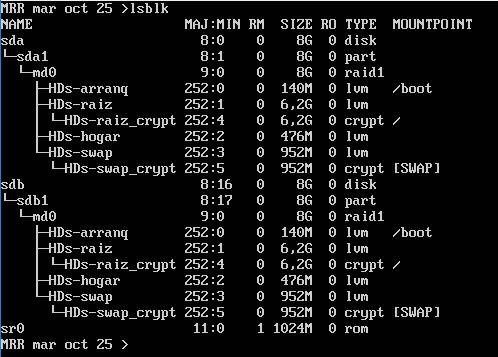
\includegraphics[scale=0.6]{figuras/ejercicio10.png} 
		\caption{Particionado del disco} 
		\label{fig:figura10}
	\end{figure}


%----------------------------------------------------------------------------------------
%	Cuestión 11
%----------------------------------------------------------------------------------------
\section{Prueba del RAID de Linux}
\subsection{\emph{\textbf{¿Cómo ha hecho el disco 2 “arrancable”?}}}

Con el comando \textbf{grub-install /dev/sdb1}

\subsection{\emph{\textbf{¿Qué hace el comando grub-install?}}}

Este comando instala un nuevo gestor de arranque en la unidad que se le especifique.


%----------------------------------------------------------------------------------------
%	Cuestión 12
%----------------------------------------------------------------------------------------
\section{Versiones de Windows Server}
\emph{\textbf{¿Qué diferencia hay entre Standard y Datacenter?}}

Una diferencia que existe entre ellas es el número de máquinas virtuales que pueden ser ejecutadas por cada una. Para la versión Datacenter no hay límite en el número de máquinas virtuales, como máximo ejecutadas en dos procesadores. 
Por otro lado, la edición Standard solo permite la ejecución de dos VMs a la vez en hasta dos procesadores. \cite{link12}

\begin{figure}[H] %con el [H] le obligamos a situar aquí la figura
	\centering
	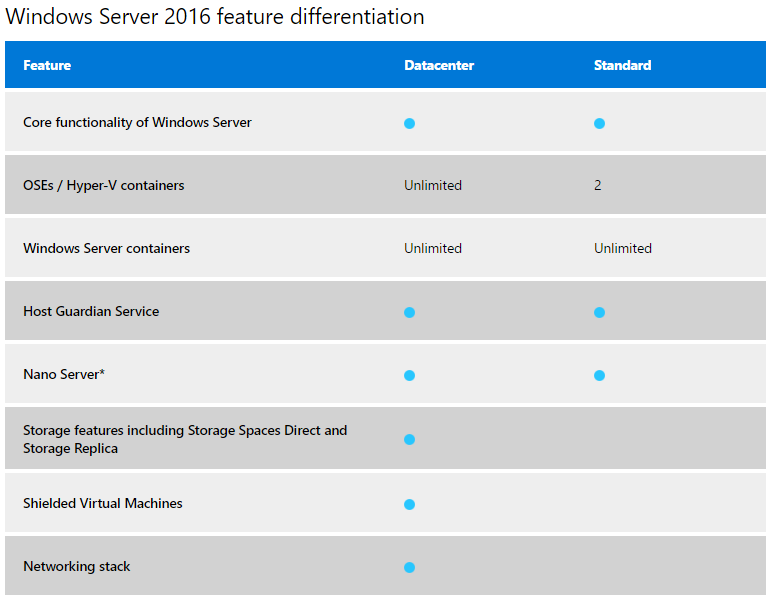
\includegraphics[scale=0.7]{figuras/ejercicio12.png} 
	\caption{Diferencias entre Standard y Datacenter \cite{figura12}} \label{fig:figura12}
\end{figure}

Como se puede apreciar en la Figura \ref{fig:figura12} hay tres características más que no
comparten ambas ediciones, siendo solamente exclusivas para la licencia Datacenter. Éstas son: \cite{link12}

\begin{itemize}
	\item Características especiales de almacenamiento, como espacios de almacenamiento directo y almacenamiento con réplica de datos.
	\item Máquinas virtuales blindadas
	\item Pila de red
\end{itemize}

\newpage
%----------------------------------------------------------------------------------------
%	Cuestión 13
%----------------------------------------------------------------------------------------
\section{Definición del RAID1 para Windows Server}
\emph{\textbf{Continúe usted con el proceso de definición de RAID1 para los dos discos de 50MiB que ha creado. Muestre el proceso con capturas de pantalla \footnote{Abrir archivo con Safari (MacOS) o Firefox si se tiene problemas con Adobe Reader.}}}

\begin{figure}[H]
	\begin{center}
		\includemovie[poster,text={\small(Pulse para ver)}]{12cm}{10cm}{figuras/particion.mp4}
	\end{center}
\end{figure}

\newpage

%----------------------------------------------------------------------------------------
%	Cuestión 14
%----------------------------------------------------------------------------------------
\section{Tipos de conexión VMSW}
\emph{\textbf{Explique brevemente qué diferencias hay entre los tres tipos de conexión que permite el VMSW para las Mvs: NAT, Host-only y Bridge.}}

La diferencia entre los tres tipos de conexión que permite el VMSW es que mientras que el modo Bridge reproduce exactamente otro nodo de la red física, en Nat la actividad de red es cubierta como si viniera del sistema operativo anfitrión y en Host-only sólo se permiten operaciones de red con el sistema operativo anfitrión.\cite{link1}

Es decir, en NAT igual que en una red doméstica con router inalámbrico, la máquina virtual será alojada en una subred independiente, por lo que puede acceder a la red exterior como su anfitrión. Sin embargo, no es posible acceder desde el exterior a ella directamente porque está protegida.

Por otro lado, en Bridge la máquina virtual estará en la misma red que su anfitrión. Eso hace que pueda tener acceso a todos los equipos de la red de acogida.

Muy distinto a lo que ocurre en Host-only, en el que a la máquina virtual se le asigna una dirección IP pero no es posible que otros equipos puedan acceder a ella.\cite{link2}

%----------------------------------------------------------------------------------------
%	Cuestiones opcionales
%----------------------------------------------------------------------------------------
\section{Cuestiones opcionales}
\subsection{\emph{\textbf{Muestre (con capturas de pantalla) cómo ha			comprobado que el RAID1 funciona.}}}
	\begin{figure}[H] %con el [H] le obligamos a situar aquí la figura
		\centering
		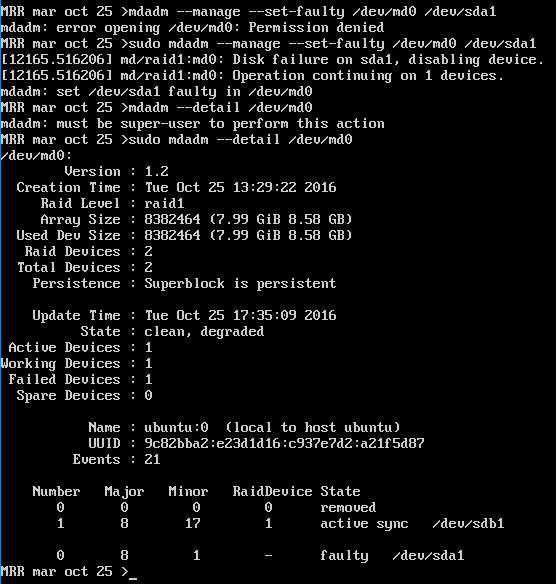
\includegraphics[scale=0.6]{figuras/ejercicio11.png} 
		\caption{Simulación de fallo en una unidad de RAID por software} 
		\label{fig:figura9}
	\end{figure}

	\begin{figure}[H] %con el [H] le obligamos a situar aquí la figura
		\centering
		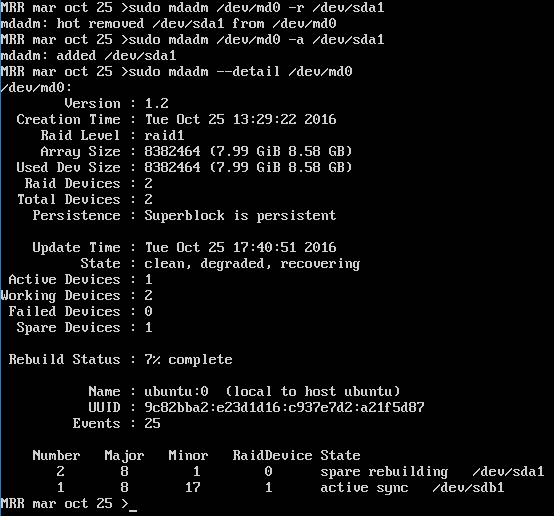
\includegraphics[scale=0.7]{figuras/ejercicio11-2.png} 
		\caption{Retirada del disco en caliente y restauración} 
		\label{fig:figura11-2}
	\end{figure}

	\begin{figure}[H] %con el [H] le obligamos a situar aquí la figura
		\centering
		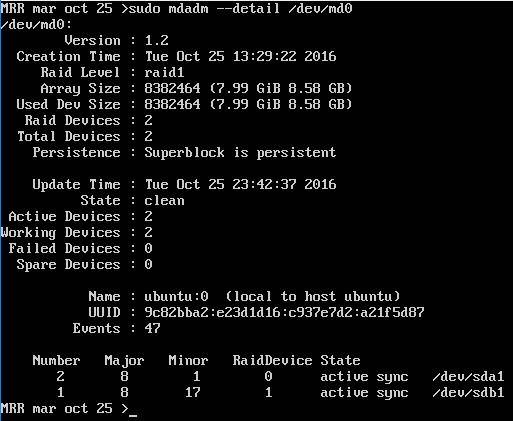
\includegraphics[scale=0.75]{figuras/ejercicio11-3.png} 
		\caption{Reconstrucción del sistema completada} 
		\label{fig:figura11-3}
	\end{figure}

\newpage
%----------------------------------------------------------------------------------------
%	Referencias
%----------------------------------------------------------------------------------------
%------------------------------------------------

\bibliography{citas} %archivo citas.bib que contiene las entradas 
\bibliographystyle{plain} % hay varias formas de citar

\end{document}
